\documentclass[a4paper,11pt]{article}
\usepackage[osf]{mathpazo}
\usepackage{ms}
\usepackage[sort&compress]{natbib}
\raggedright

\usepackage[colorinlistoftodos]{todonotes}

\title{\texttt{TREE}: A package for modelling plant TRait Ecology and Evolution}
\author{Daniel S. Falster, Richard G. FitzJohn, and Mark Westoby}
\affiliation{
Department of Biological Sciences, Macquarie University, Sydney, NSW 2109, Australia\\
Email for correspondence: \texttt{daniel.falster@mq.edu.au}\\
A manuscript in consideration as a research paper for
publication in MEE as part of the Special Feature \emph{Demography
  beyond the Population}.}
\date{}

\bibliographystyle{mee}

\usepackage[title,titletoc,toc]{appendix}

\mstype{Applications Note}
\runninghead{TREE}
\keywords{demography, emergent, fitness, growth,
physiology, metapopulation, mortality, reproduction, size-structure,
tradeoff}

\begin{document}
\mstitlepage
\noindent
\parindent=1.5em
\addtolength{\parskip}{.3em}
\doublespacing
\linenumbers
\section{Summary}\label{abstract}
\begin{enumerate}
\def\labelenumi{\arabic{enumi}.}
\itemsep1pt\parskip0pt\parsep0pt
\item
  Population dynamics in forests are strongly size-structured:
  larger plants shade smaller plants while also expending
  proportionately more energy on building and maintaining woody stems.
  Although the importance of size-
  structure for demography is widely recognised, many mechanistic models
  either omit it entirely, or include only coarse approximations.
\item
  Here we introduce the \texttt{TREE} package (TRait Ecology and Evolution), an
  extensible framework for modelling plant demography across the entire
  life cycle and in structured metapopulations, via coupled differential equations.
  At its core, \texttt{TREE} is an
  individual-based mechanistic model where plant physiology and demography is mediated by
  traits. Individuals from multiple species can be grown in isolation,
  in patches of competing plants, or in metapopulations under a
  disturbance regime. Dynamics within patches of competing plants are
  resolved using novel extensions of the Escalator Boxcar Train
  technique. Combined effects of trait-, size- and patch-structured
  dynamics are integrated into population level estimates of
  reproductive fitness.
\item
  \texttt{TREE} is presented as an open source \texttt{R} package and is
  available at
  \href{https://github.com/traitecoevo/tree}{github.com/traitecoevo/tree}.
  While accessed from R, the core routines in \texttt{TREE} are written in C++.
  The package provides for alternative physiologies and for
  hyper-parameterisation on the basis of plant functional traits. A
  detailed test suite is provided to ensure correct behaviour of the code.
\item
  We provide worked examples illustrating \texttt{TREE}'s use to study the
  influence of functional traits on growth of individual plants, of
  whole patches and on assembly of ecological communities.
\end{enumerate}

\section{Introduction}\label{introduction}

Plant growth and demography are fundamentally size- and trait- structured,
influencing dynamics over time-scales ranging from instantaneous physiological
effects to long-term evolutionary outcomes \citep{Harper-1977, Westoby-2002}. As
an individual increases its leaf area, its potential to generate
photosynthate also rises. Yet as individuals get larger, an increasing
fraction of that photosynthate is diverted towards
building and maintaining support tissues
\citep{Givnish-1988, Enquist-2007} and reproduction \citep{Thomas-2011}. Consequently 
rates of growth and mortality change with individual size
\citep{Muller-2006, Thomas-2011, Ruger-2011, Wright-2010}. The traits of
a species also interact with size to shape its demography. Leaf
construction costs and wood density affect growth rates
\citep{Wright-2010}. Other traits such as seed size and height at
maturation determine start and end points of ontogenetic trajectories
\citep{Westoby-2002}. Over longer time-frames, natural selection generates
traits that amplify size-related effects on demography,
such as faster growth, larger seeds or taller height \citep{Falster-2003}. 
Accounting for the effects of size and traits in models is therefore fundamental to developing theory on the structure and dynamics of the biosphere
\citep{Purves-2008, Moorcroft-2001, Falster-2003}, in particular for notable
phenomena such as successional dynamics, self thinning, trait evolution
and species coexistence.

Although the importance of size-structure for vegetation function and
demography has been long been recognised
\citep{Harper-1977, Hara-1984, Shugart-1980, Huston-1987, Moorcroft-2001,
Kohyama-1993, Enquist-2007, Pacala-1996, Coomes-2007},
most large-scale mechanistic models of plant growth either omit it
entirely, or only include coarse approximations
\citep{Cramer-2001, Dekauwe-2014, Kelley-2013, Sitch-2003}. The likely
reason is the computational
challenge of modelling size-structured dynamics. During the 1980s and
early 1990s, size-structured ``gap'' models were widely used
\citep[e.g.][]{Huston-1987, Shugart-1980}. These gap models were
parameterised in terms of growth using statistical functions; this meant 
that data had to be collected for each species, limiting widespread application. 
The next generation of models focussed on establishing core physiology for 
a limited number of functional types, and, presumably for computational reasons,
sacrificed details of demography in order to achieve global coverage
\citep{Haxeltine-1996,Woodward-1995}. This history has brought us to the
current perplexing situation where all but a couple
\citep[e.g.][]{Moorcroft-2001, Smith-2014} of the most popular vegetation
models lack size-structure. Instead, most models
are focused on modelling fluxes carbon and water, but say little about
demographic behaviour, and consequently are also unable to account for
any non-linear demographic feedbacks that may arise.

Interestingly, most models used in theoretical ecology to explore
questions about species coexistence also lack size-structured dynamics
\citep[e.g.][]{Calcagno-2006, Geritz-1995, Leimar-2013, Levin-1974,MacArthur-1967,Tilman-1985}.
It is common to assume competitive interactions are influenced by
size-related traits such as adult size and seed size, but detailed
size-structured demography is rarely considered, at least for plant
models \cite[for animal examples, see][]{Deroos-1988, Deroos-1992}. Consequently, it has
been difficult to connect mechanisms described in these simplistic
models with type of data often collected in the field, such as physiological
leaf traits, and demographic data on growth and mortality in long-term monitoring 
plots \citep{Adler-2013}.

In this note, we describe the \texttt{TREE} package for R
\citep{R-2015}, a mechanistic framework for studying the effects of size
structure and trait variation on the demography of individual plants, of
patches of competing plants, and of meta-populations structured by a
prevailing disturbance regime. The package came about as a way to extend
previous work investigating the effect of traits on vegetation
properties and the mechanisms facilitating
coexistence of trait mixtures \citep{Falster-2011,Falster-2015}. Building 
on earlier studies \citep{Deroos-1997,Kohyama-1993,Moorcroft-2001}, these
papers outlined methods for driving trait-, size- and patch-structured 
dynamics from a core physiological model. Here we provide 
a robust and extensible implementation of those methods. 
We describe the general approach of the
package and then sections with details at different levels of
ecological organisation. Each section provides a short description of
the required methods, design considerations, and then 
example applications. Detailed
technical documents are provided as supplementary information (see Appendices),
and updated versions of technical documents are also available within the \texttt{TREE}
package itself. 

While the applications highlighted reflect our own interests in understanding
trait-based demography and community assembly, we expect the methods provided
to be useful in variety of contexts. For example, prior to \texttt{TREE} there
was no \texttt{R} package that allowed one to simply grow a plant over time,
based on well-understood physiology. Surely this is one of the simplest
demographic actions one might hope for, with diverse potential applications in
ecology, evolution, forestry, agriculture, and vegetation modelling. More
specifically, \texttt{TREE} provides a  platform for investigating how
morphological and physiological traits influence  growth rate and shade
tolerance, thus potentially giving a theoretical foundation  for observed
empirical patterns \citep{Wright-2010,Baltzer-2007}. Being driven by traits,
the model can be extended to potentially very many species. Users can also 
add their own physiological models. Individual plants
can then be  situated in a patch with competitors and the demography of a
competing population  investigated, thereby capturing phenomena such as multi-
species self-thinning,  successional transitions and age-related changes in
vegetation productivity. \texttt{TREE}  models the emergent behaviour of
patches deterministically, based on a continual  size-density distribution. As
such, it is not required to specify a particular patch size.  Finally,
\texttt{TREE} allows for emergent phenomena across a metapopulation of patches
to  be investigated, and thus provides a tractable mechanism to scale from
individual plant to  vegetation, incorporating the non-linear effects of size
and traits on vegetation outcomes. In  this sense \texttt{TREE} is similar to
the Ecosystem Demography \citep{Moorcroft-2001}  and LPJ-GUESS
\citep{Smith-2014} models. However, whereas these other models were designed
to primarily capture large-scale regional biogeocehcmisty driven by climatic
variables,  \texttt{TREE} was designed so that the rules driving the
demography of individual trees, patches and metapopulations could be
manipulated and studied in detail. The three models are therefore highly 
complimentary, and also connect with the increasingly sophisticated statistical 
methods now available to analyse size-structured data \citep[e.g.][]{Metcalf-2013}.

\section{The approach}

\texttt{TREE} is a mechanistic model, meaning the dynamics of the system arise
from rules specifying how individuals grow and interact. In ecology,
there is a long history of using simple deterministic models
to understand biological phenomena, such as Lotka-Volterra population dynamics
\citep{MacArthur-1967, Leimar-2013} .
\texttt{TREE} was developed with this style of analysis in mind, while also
allowing for a richer set of ecological dynamics than is possible in
population models lacking size structure. The package implements methods
for physiological, population, and adaptive dynamics (Fig.
\ref{fig:schematic}) following methods described by \citet{Falster-2011}
and \citet{Falster-2015}. The core rules in \texttt{TREE} are about the
short-term physiological functioning of an individual plant and how
these are influenced by its traits, size and light environment. Dynamics
at higher levels of organisation then arise as emergent properties,
driven by growth physiology, competition for light and disturbance (Fig.
\ref{fig:schematic}). Demographic phenomena can be studied at the three
levels: individual plants, stands of competing plants, and entire
metapopulations.

\section{Effects of size, trait and environment on demography of individual plants}

The core of \texttt{TREE} is a model for a plant's physiological strategy as
specified by its traits (Fig. \ref{fig:schematic}a). This sub-model
estimates rate of biomass production for a plant, given its size, light
environment, and the supplied physiological constants. Gross photosynthetic 
income is
estimated from total leaf area and the light distribution across the
plant's canopy. Costs of tissue respiration and turnover are then
subtracted. The remaining biomass is then allocated between growth and
reproduction. The strategy model thus includes a list of physiological
rules and associated parameters.

The core job of the physiological model is to take size, light
environment and physiological parameters as inputs, and to return growth rate,
mortality and fecundity as outputs, in other words to move from
individual growth to demography. However additional quantities are also
available as output, such as total assimilation and the respiration,
turnover, and allocation rates for different tissues.

The default physiological model used in \texttt{TREE} largely reflects that
presented in \citet{Falster-2011}, but with extensions allowing for diameter
growth also to be estimated. To properly model trait variation,
different parameters (such as rates of leaf turnover, respiration, photosynthesis 
per leaf area) in the model are linked via assumed tradeoffs. For
example, the trait LMA is used to estimate the rate of leaf turnover,
based on observed scaling relationship spanning across diverse vegetation and
plant functional  global \citep{Wright-2004} (see 
Appendix \ref{sec:FFW16} for details).

\subsection{Design features}

\texttt{TREE} includes a default physiological model (fully described and derived
in the Appendix \ref{sec:FFW16}). However a feature of the package is that alternative
physiologies can be used, and the parameters of each model can be
altered. Trait differences are accounted for by altering relevant
parameters (see Appendix \ref{sec:parameters}).

\subsection{Applications}

With above functionality, \texttt{TREE} can be used to estimate essential
physiological rates for individual plants (Fig. \ref{fig:plant}). The
function \texttt{grow\_plant\_to\_size} takes a given strategy and light
environment and grows the plant, producing a trajectory of size over
time (Fig. \ref{fig:plant}a). This is achieved by integrating an
Ordinary Differential Equation (ODE) of size-dependent growth rate (see
Appendix \ref{sec:demography} for more
details). As the plant grows, allocation to different tissue types varies, and
the composition of the plant changes to include more stem and less
leaf (Fig. \ref{fig:plant}b). This in turn affects maintenance and
turnover costs and the growth rate of plants (Fig. \ref{fig:plant}c).
This shift in allocation alone generates a distinctive hump-shaped pattern of absolute
growth with size \citep{King-2011}, and equally the widely regarded
decline in relative growth rate with size from birth onwards
\citep{Enquist-2007}.

By varying the light environment and measuring growth rate, the whole
plant light compensation point (WPLCP) can be computed (Fig.
\ref{fig:plant}d). The WPLCP is the light level at which the plant 
stops growing, and is increasingly regarded as the most useful
measure of a strategy's shade tolerance
\citep{Givnish-1988, Baltzer-2007, Lusk-2013}. As expected, WPLCP
increases with plant size, due to increased costs of building and
maintaining stem and leaf tissues \citep{Givnish-1988}. Likewise, WPLCP
decreases with LMA, because high LMA species have lower leaf turnover
\citep{Baltzer-2007, Lusk-2013}.

\section{Plants competing in a patch}

Within patches of competing plants, competition for light generates
strong non-linear feedbacks on growth, survival and reproduction. In the
\texttt{FFW16} physiological model, we consider only the effect of
shading on rates of biomass production, although competition for other
resources such as nitrogen or water could also be considered with
suitable extensions.

Modelling the development of a competitive hierarchy within a patch
requires that both the initial size distribution and the inflow of new
recruits be specified. We have primarily been interested in dynamics of
a patch recovering from disturbance, and have therefore started with an
empty patch and constant flow of seeds from a global seed rain (Fig.
\ref{fig:schematic}b).

\subsection{Design features}

When modelling a patch, we are interested in modelling changes in the
size-density-distribution \(n(x,h,a)\) with patch age \(a\), i.e. the density of
individuals with traits \(x\) and height \(h\) within a patch of age \(a\). Density
is measured as individuals per unit height and per unit ground area.

We assume that patches are large, and are vertically but not horizontally
structured. In other words, we account for size differences but not spatial 
layout within the patch. Similar assumptions are found in many models
simulating size-structured dynamics
\citep{Moorcroft-2001, Huston-1987, Smith-2014,Kohyama-1993}. The assumption of a large
patch means the population of plants within the patch -- and thus the 
dynamics of \(n\) -- behave deterministically \citep{Deroos-1997}, and can therefore be
approximated via a Partial Differential Equation (PDE) (see Appendix
\ref{sec:demography}). The same PDE has been shown to capture average behaviour
across a large number of small patches \citep{Moorcroft-2001}. The model may 
therefore capture average demographic behaviour across a range of patch sizes.

Ideally one would also consider spatial interactions within patches,
however such models are very computationally demanding, and also
impossible to solve in a deterministic fashion \citep{Huston-1987, 
Pacala-1996}.
Moreover, it remains unclear whether resolving spatial details within a
patch would provide further ecological detail, in part because the
process of competitive thinning tends to break down spatial clusters
\citep{Strigul-2008}.

Our approach for modelling size-structured population dynamics
is based on the Escalator Boxcar Train technique (EBT)
\citep{Deroos-1997, Deroos-1992, Deroos-1988}. The EBT solves the PDE
describing development of \(n\) by approximating the density function
with a collection of cohorts spanning the size spectrum. Following a
disturbance, a series of cohorts are introduced into each patch. These
cohorts are then transported along the characteristic equations of the
PDE. Biologically these are the growth trajectories of individuals,
conditioned on them surviving (e.g. Fig. \ref{fig:patch}a). Meanwhile,
growth and mortality combine to alter the density of individuals along
the trajectories (Fig. \ref{fig:patch}b).

We introduce two extensions to the EBT: i) a new method for estimating
the size-density distribution, and ii) a technique for handling strong
size-asymmetric competitive feedbacks, such as occur under strong
competition for light. The original EBT
\citep{Deroos-1997, Deroos-1992, Deroos-1988} proceeds by approximating
the first and second moments of the density distribution \(n\) within
each cohort. In \texttt{TREE} we use a different -- but from a theoretical
perspective equally valid --  approach. Instead of tracking first and second
moments of the size-distribution within cohorts, we track a point mass
estimate of \(n\) along the trajectory for the boundary
of each cohort. We found this approach preferable because it does not
require us to maintain a separate set of equations for the smallest
cohort \citep{Deroos-1997}.

The extension for handling strong size-asymmetric competition involves
adaptive refining of time points at which new cohorts are introduced
into the population. In the original EBT, cohorts were introduced at a
fixed time interval. Under competition, the growth trajectories of
individuals born at similar times can diverge substantially over time
(Fig. \ref{fig:patch}a; Appendix \ref{sec:demography}).
This is can become a problem later during patch
development because much of the population can be located between
widely-spaced cohorts, delivering low numerical precision. To maintain
numerical precision we therefore use an iterative algorithm to adaptively refine
the cohort spacing until the trajectories of adjacent cohorts remain
adequately resolved throughout development of the patch (see
Appendix \ref{sec:demography} for details). This refinement causes an uneven
distribution of cohort introduction times across patch age (Fig.
\ref{fig:patch}a), generally with tighter spacing of cohorts in 
younger patches.

\subsection{Applications}

Modelling of size-structured dynamics via solving of a deterministic PDE
enables multiple complex non-linear demographic phenomena to be
investigated.

First, \texttt{TREE} can simulate patterns of patch development after
disturbance, including self-thinning behaviours and successional
replacement. Whereas previous approaches for modelling self-thinning
were limited to a single species
\citep[e.g.][]{Barnes-2004, Coomes-2007}, \texttt{TREE} accommodates multiple
 species with different traits (Fig. \ref{fig:schematic}b; Fig.
\ref{fig:patch}).

Second, \texttt{TREE} allows for the effects of competition and succession on
productivity and biomass accumulation within a patch to be investigated
\citep{Falster-2011}. Leaf area cover and rates of biomass production
tend to vary with patch age. Such changes might come about via a
combination of physiological and structural changes
\citep{Binkley-2002, Smith-2001, Ogawa-2010, Coomes-2007}. \texttt{TREE} enables
the effects of competitive feedbacks to be incorporated, in addition to
any intrinsic physiological factors. Moreover, \texttt{TREE} allows for the
contributions of different species to be mapped (Fig. \ref{fig:patch}c).

While many vegetation models still lack size structure, the importance of
size-structure for modelling phenomena such as allocation and production is
being increasingly noted \citep{Moorcroft-2001, Dekauwe-2014, Falster-2011}.

\section{Trait, size and patch structured vegetation}

Most vegetation is subject to a disturbance regime, such that patches of
the landscape are cleared at some rate, by fire, cyclone, landslide, or
disease outbreak
\citep{Connell-1978, White-1979, Chambers-2013, Bormann-1979, Clark-1991, Coomes-2007}.
The vegetation thus comprises a collection of patches differing in time
since last disturbance and linked via seed dispersal (Fig.
\ref{fig:schematic}b). Such a system is often refereed to as a
structured metapopulation \citep{Gyllenberg-2001}.

\subsection{Design features}

Having simulated a single patch, it is straightforward to scale up from
a single patch to an entire metapopulation, at least for the situation
of metapopulations at an equilibrium mix of patch ages and where
disturbances remove all established vegetation. The frequency-density
\(p(a)\) of patches aged \(a\) in the landscape is needed. Assuming there
are a large number of patches means the dynamics of \(p\) behave
deterministically and can be approximated via a second PDE
\citep{Vonfoerster-1959, Mckendrick-1926} (see Appendix
\ref{sec:demography} for
details). Scaling from patch to metapopulation is then achieved by
weighting the temporal dynamics of a single patch by \(p(a)\), the
relative abundance of patches aged \(a\) in the metapopulation.

The main numerical challenge in stepping from single patch
to metapopulation is to identify the equilibrium seed rain of the
metapopulation. For a given seed rain input, the model produces a seed rain output. 
The equilibrium seed rain is the vector of seed rain
where input seed rain equals output seed rain. Finding this equilibrium
requires finding a root of a multidimensional function, subject to the
constraints that this root is stable (e.g., the trivial equilibrium of
zero seed rain always exists, but is often not stable) (Appendix \ref{sec:fitness});

\subsection{Applications}

As previously noted \citep{Kohyama-1993, Moorcroft-2001, Falster-2011} a
feature of the size-structured metapopulation concept implemented here
is that it reconciles equilibrium and non-equilibrium approaches to
modelling ecological dynamics
\citep{Levin-1974, Bormann-1979, Connell-1978, Coomes-2007}. An
equilibrium may be approached at the level of metapopulation, meaning
the seed rain and size structure across the entire metapopulation is
approximately stable. Yet the structure of vegetation within individual
patches is constantly in flux. Patches continue to age and their
residents continue to grow until they are disturbed.

Beyond its conceptual appeal, this idea of a dynamic equilibrium allows
us to close the demographic feedback loop and thereby create a
self-regulating system. The equilibrium seed rain for multi-species
communities is approached demographically, incorporating the combined
effects of the model's physiological rules, species traits, competitive
interactions and the prevailing disturbance regime on the
size-distributions of plants within a metapopulation of patches. Unlike
some vegetation models, there is no need to set the density of seeds or
seedlings, these arise as outputs from the model. Characteristics of the
vegetation such as total leaf area, biomass, productivity and allocation
to different plant parts also arise as emergent properties (Fig.
\ref{fig:patch}c). Similarly, distributions of abundance, leaf area and
growth rate with respect to size emerge at both patch scale and scale of
metapopulation (Fig. \ref{fig:emergent}). Note in particular how a single
physiological model produces a variety of height-density relationships, 
dependent on patch age, as well as an emergent average across all patches 
(Fig. \ref{fig:emergent}). This emergent relationship might then be 
compared to the observed distributions in large forest plots \citep{Muller-2006}.

\section{Invasion fitness}

With the extension to metapopulation, we are modelling demography across
the entire life cycle and are thus in a position to estimate the fitness
of different types. Invasion fitness quantifies the ability of a rare
individual with particular traits to establish in a community of
established residents at their equilibrium densities \citep{Metz-1992}.
Invasion fitness
is ideally calculated as the long-term per capita growth rate of the new
type; however, in structured metapopulations, a more convenient
indicator of per-capita growth rate is given by the logarithm of the
basic reproduction ratio \citep{Gyllenberg-2001, Metz-2001}. The basic
reproduction ratio \(R\) is simply the total seed output of the new
type, averaged across the metapopulation. The new type can invade when
\(R > 1\).

\subsection{Applications}

With fitness defined, it becomes possible to model adaptive dynamics
and community assembly \citep{Dieckmann-2007, Geritz-1998}. This is best
thought of as occurring on a fitness landscape, a surface with fitness
plotted against one or more species traits (Fig. \ref{fig:fitness}). The
reproductive success of individuals possessing a particular trait value
is measured in the size- and patch-structured metapopulation, and
depends on both the traits and densities of other species in the current
resident community. The reason this is interesting is that under
frequency- and density-dependence, evolution tends to favour different
trait mixtures compared to those predicted by models that optimise some
feature of the community, such as total biomass or carbon production or
seed production in the absence of competition
\citep{Falster-2003, Dieckmann-2007}.

Fitness landscapes will be positive in regions that allow invasion, and
zero for species that are at equilibrium. The slope of the fitness
landscape at a resident indicates the direction of selection; a negative
slope (dashed line in Fig. \ref{fig:fitness}a) indicates selection for
smaller trait values. Fitness landscapes are constantly reshaped
as species are introduced and evolve, reflecting the non-linear
demographic feedbacks that occur under frequency-dependent evolution
 \citep{Geritz-1998,Dieckmann-2007}. Following the fitness gradient, can lead to an
evolutionary branching point \citep{Geritz-1998,Dieckmann-2007};
at this point there is no directional selection (solid line in
figure \ref{fig:fitness}a) but invasion is possible both above and below
it in trait space. It is often possible
to find a configuration where fitness is negative everywhere (solid line
in Fig. \ref{fig:fitness}b) except for the zero points where species are
present. This community is immune to invasion from any other strategies
\citep{Geritz-1998}.

Identifying conditions promoting trait diversity is a valuable use-case
for \texttt{TREE}. Coexisting plant species differ in a range of physiological
traits, yet the conditions allowing for these different types to coexist
in face of competition for a common set of resources remain largely
unknown. The simple example here can be extended to multiple dimensions
and can be used to investigate how tradeoffs facilitate coexistence
\citep{Falster-2015}

\section{Implementation details}

\texttt{TREE} is written in C++ and \texttt{R}, using the package \texttt{Rcpp}
\citep{Eddelbuettel-2011, Eddelbuettel-2013} to bridge between the two
languages. Due to the computationally intensive nature of the model, the
core physiological and demographic components are in C++ to maximise
speed. We used templated types that allow the demographic and evolutionary
components to be driven by alternative physiological models while
retaining the same interface at higher levels. Despite mostly being
programmed in C++, all components of the model, down to individual
plants, can be extracted and interacted with dynamically in R, using the
\texttt{RcppR6} package \citep{RcppR6}.

\texttt{TREE} makes use of much existing software, including the programming
language C++; the \texttt{R} computational environment \citep{R-2015}, the \texttt{R}
packages \texttt{Rcpp} \citep{Eddelbuettel-2011, Eddelbuettel-2013},
\texttt{R6}\citep{Chang-2014}, and \texttt{testhat}
\citep{Wickham-2011}; and the Boost Library for C++
\citep{Schaling-2014} via the \texttt{R} package \texttt{BH}
\citep{Eddelbuettel-2015}. Source code is hosted at
\href{https://github.com/traitecoevo/tree}{github.com/traitecoevo/tree}.
Installation instructions are available at this homepage, and binary
releases will also be available there.

The current parametrisation of the physiological model is based on
\citet{Falster-2011}. Parameter values were drawn from available literature (see
Appendix \ref{sec:FFW16}); however for some parameters limited or no data were
readily available. Providing updated parameter sets is trivial; the challenge 
is to infer suitable values by constraining  outputs from \texttt{TREE} against diverse data sources
\citep{Lebauer-2012, Keenan-2013}. This is an area in which we are still actively working.

\section{Closing comments}

The \texttt{TREE} package makes it easier for researchers and forest practitioners
alike to investigate a variety of non-linear demographic phenomena.  Rather
than provide a model with a few routines, we have developed an extensible
framework that we hope can be used to answer a number of questions at a
variety of scales. The specific use-cases highlighted here arise from our
interest in the assembly of trait mixtures in communities. However a variety
of other uses would be possible, and also extensions to address other facets
of community assembly. For example,  the physiology of growth could be
modified to account for rising atmospheric CO2 or the effects of competition
for multiple resources could likewise be investigated.

It is hoped that the approach here can be used to inform both future empirical
research and model development in neighbouring areas. As noted above, most
large-scale mechanistic models of plant growth do not explicitly model size
structure, so remain unable to investigate demographic phenomena
\citep{Cramer-2001, Dekauwe-2014, Kelley-2013, Sitch-2003}. At the same time,
much attention is paid to detailed leaf-level physiology. \texttt{TREE} aims to bridge
this gap that emerged in the model landscape, where detailed physiology and
size-structured dynamics combine to drive forest structure and function via
traits.

\section{Acknowledgements}

DS Falster was supported by an ARC discovery grant (DP110102086). RG
FitzJohn was supported by the Science and Industry Endowment Fund
(RP04-174). M Westoby was supported by a fellowship from Australian
Research Council.

\clearpage
\bibliography{refs}

\clearpage

\section{Figures}\label{figures}

\begin{figure}[h!]
\centering
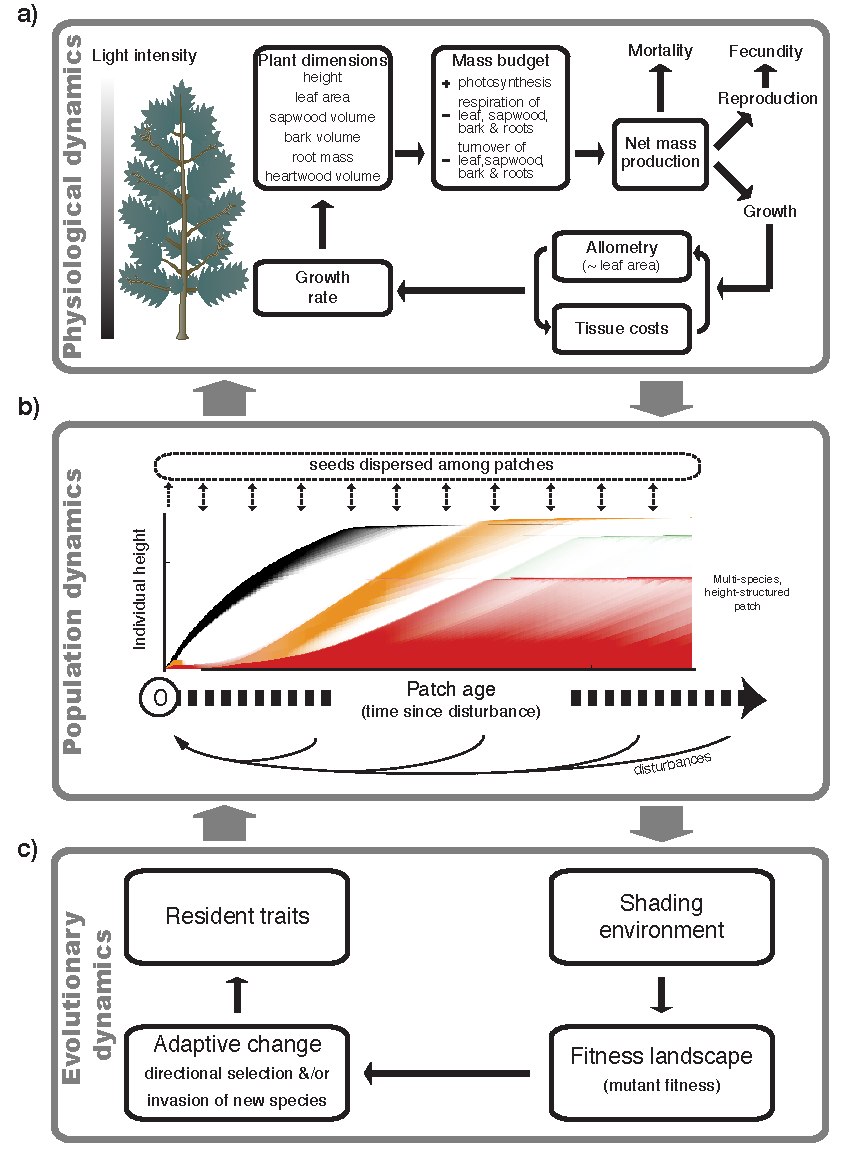
\includegraphics[width=15cm,height=15cm,keepaspectratio]{figures/schematic}

\caption{Processes modelled within \texttt{TREE} include physiological, population, and
evolutionary dynamics.
Dynamics across all three levels are driven by the
physiological sub model determining an individual's physiological and
demographic rates on the basis of its traits, size and light environment (a).
(b) Competitive hierarchies  are modelled by tracking the height distribution of
individuals across within a "patch" after a disturbance. The intensity
of shading indicates the density of individuals at a given height for
different species (distinguished by colours). A size- and patch-structured
metapopulation consists of a distribution of patches linked by seed dispersal.
Disturbances occasionally remove all vegetation within a patch, resetting the
patch. (c) The traits of the resident species determine the shading environment
across the metapopulation, which in turn determines the fitness landscape.
Resident traits adjust through directional selection up the fitness landscape
and through the introduction of new species. Adapted from
\citet{Falster-2011}, \citet{Falster-2015}. }

\label{fig:schematic}
\end{figure}

\newpage

\begin{figure}[h!]
\centering
\includegraphics[width=15cm,height=15cm,keepaspectratio]{figures/plant.pdf}
\caption{Physiological dynamics for individual plants vary with size, trait
and light environment. (a) Growth trajectories for plants differing in light
environment and trait (LMA, low = 0.1, solid line; high =  0.267, dashed
line). Lower light environments slow trajectories and interact non-linearly
with traits. (b) Over time, the fraction of living tissue switches from leaf
towards sapwood, with high LMA species having relatively more mass in leaf
than low LMA species. (c) Growth rates peak around 5m high, but this position
varies with both trait and light level (note that this is the derivative of
panel (a)). (d) Growth rates vary with plant size (seedling and mature shown)
and with traits; growth rate differences are more pronounced in high light.
Whole plant light compensation points emerge from the model as the point where
growth rate is zero (x intercept).  The light level used in panels (a) and (c)
is indicated with dots.} [Could you put delta symbols on the y axis rather than d? Also there is alot going in these figures with 4 lines each. You could make it easier for the reader by adding the dashed lines to the keys]
\label{fig:plant}
\end{figure}

\newpage

\begin{figure}[h!]
\centering
\includegraphics[width=15cm,height=15cm,keepaspectratio]{figures/patch.pdf}
\caption{Population dynamics for two species competing within a patch. Lines
in panels (a) same growth trajectories for individuals on the
boundary of successive "cohorts" for each species, using a schedule of 
introduction times generated by an adaptive refinement algorithm.
 Red lines are the low LMA
species from figure \ref{fig:plant}, blue lines are the high LMA species.  The
initial growth rate advantage of the low LMA species (see Figure
\ref{fig:plant} c) means it quickly over tops the high LMA species,
suppressing its growth.  Self-thinning leaves space for the high LMA species
to establish below the canopy of the fast species. Panel (b) shows the same
trajectories as in panel (a), but with shading indicating the density $n$ of
individuals at given size and patch age (light = low density, dark = high density).  
(c) The leaf area index at ground
level for each species.  The dotted line is the total leaf area index (sum
across both species).}
\label{fig:patch}
\end{figure}

\newpage

\begin{figure}[h!]
\centering
\includegraphics[width=15cm,height=15cm,keepaspectratio]{figures/emergent.pdf}
\caption{Emergent size-distributions across a metapopulation.
Grey lines show patterns within individual patches differing in time since disturbance (age), with blue lines indicating patches of a specific age. Panels show (a) patterns of abundance, (b) leaf area and (c) height growth rate against size. Note that units of panels (a) and (b) are per unit height and per unit ground area, respectively.}
\label{fig:emergent}
\end{figure}

\newpage

\begin{figure}[h!]
\centering
\includegraphics[width=15cm,height=15cm,keepaspectratio]{figures/fitness.pdf}
\caption{Example fitness landscape for LMA, showing potential for stable
coexistence of multiple types.  Fitness is the log of the population growth
rate - at zero species are at equilibrium, above zero they will increase in
density.  (a) Landscape generated by a single species.  At LMA of 0.1 (the
dashed line) there is directional selection for smaller LMA.  At LMA of 0.08
(solid line) there is a branching point (see inset for more detail).  (b)
Landscape generated by two species, holing the first at LMA of 0.08.
Introducing a species at the maximum fitness value from panel (a) reduces the
region of positive fitness considerably (dashed line).  Dotted lines show
subsequent invasions and replacements of the second species, and the solid
line shows a stable fitness landscape where both species exist on a peak in
the fitness landscape.  At this point no further invasion is possible.}
\label{fig:fitness}
\end{figure}

\clearpage

\begin{appendices}\label{sec:appendices}

\section{Default physiological model for \texttt{TREE}}\label{sec:FFW16}

See attached file \url{tree_physiology.pdf}

\section{Modelling demography in the \texttt{TREE} package}\label{sec:demography}

See attached file \url{tree_demography.pdf}

\section{Solving for equilibrium seed rain}\label{sec:seed}

See attached file \url{vignette_equilibrium.R}

\section{Calculating fitness in the \texttt{TREE} package}\label{sec:fitness}

See attached file \url{vignette_fitness.R}

\section{Modifying parameters of physiological model}\label{sec:parameters}

See attached file \url{vignette_parameters.R}

\end{appendices}
\end{document}
